\section{Marco referencial}

\subsection{Marco teórico}

\subsubsection{Estación meteorológica}

Automatic weather stations

\subsubsection{Redes meteorológicas}

\subsubsection{API REST}

Los sistemas informáticos que se componen de más de un componente, utilizan diversos métodos de comunicación entre ellos. Desde el accesar directamente a localizaciones de memoria física o virtual en un dispositivo para compartir información hasta crear librerías compartidas entre sistemas para accesar a la información en un depósito externo (conocidas como APIs), cada forma de acceso a los datos tiene su propio nivel de abstracción, oportunidades, y desventajas, las cuales deben ser evaluadas antes de elegir una tecnología adecuada para responder a las necesidades de cada proyecto.

Un API REST es un sistema de acceso a la información de sistemas externos por medio de protocolos \textit{Web}, tales como HTTP/HTTPS, los cuáles permiten la consulta de datos en cualquier lenguaje que permita realizar conexiones y consultas a sitios web \cite{REST_API_design}. Entre las principales características de los API REST se encuentra **la falta de la necesidad** de proveer un estado para acceder a la información, esto implica que no es necesario mas que conocer la ruta en la que se encuentran los datos requeridos para acceder a ellos. Las ventajas que ofrece es la amplia disponibilidad de acceso a los datos y la fácil integración con sistemas existentes de información\cite{OpenAPI_example}.

\begin{figure}[!ht]
	\centering
	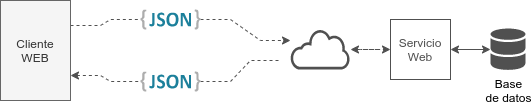
\includegraphics[width=.70\linewidth]{images/diagrams/REST.png}
	\caption{Diagrama del protocolo REST.}
	\label{fig:coms_nodos_raspberry}
\end{figure}

\subsubsection{OpenAPI}

Debido a la naturaleza libre de el desarrollo web, y la poca estandarización de la comunicación entre los clientes web con los servidores, se creó la iniciativa OpenAPI a partir de un estándar existente proveído por la compañía Smartbear, Swagger. Este estándar para la comunicación con sitios por medio de APIs REST rápidamente fué ganando popularidad gracias a la fundación Linux hasta convertirse en un estándar utilizado ampliamente por diversas organizaciones y empresas\cite{OpenAPI_foundation}.

El estándar OpenAPI es un esquema de definición de estructura de datos en JSON. En este esquema se definen las rutas a las cuáles se puede acceder, los parámetros que aceptan y sus respectivos tipos de datos, así como la información que responde y los tipos de datos de los mismos. Y debido a la naturaleza abierta del esquema, este puede ser generado e integrado nativamente con el uso de diversas tecnologías de desarrollo. Permitiendo, por ejemplo, el generar las clases e interfaces correspondientes para el uso por medio de clases de los datos para lenguajes de programación fuertemente tipados\cite{openapi_generator}

\subsubsection{Redes de comunicación}

Red Local, redes NAT y capas de NAT en el pais. Mencionar direcciones públicas

\subsubsection{Modelo OSI}

\subsubsection{VPN}

VPN (Incluir segmento sobre a seguridad involucrada en la VPN), y sobre la facilidad de conexion con SSH


\subsection{Marco tecnológico}

Esta es una descripción de las herramientas de tecnología que se utilizarán para el desarrollo del proyecto:

\subsubsection{Docker}

Docker es un sistema para la creación y distribución de imágenes de software, principalmente orientado a servidores, que permite el crear un ambiente replicable agnóstico al sistema operativo del host. Es un estándar en la industria de desarrollo de software para crear sistemas complejos manteniendo una relativa simpleza al desplegar nuevas instancias\cite{rad2017dockerAnalysis}.

Docker utiliza un sólo Kernelde linux para la creación de los contenedores y cada uno de los contenedores puede contener hasta \textit{n} procesos, lo que lo ayuda a reducir el tamaño de sistemas complejos\ref{fig:docker_diagrama}. Además de ofrecer una mayor flexibilidad y escalabilidad para tanto para realizar pruebas en máquinas de desarrollo como para distribuir y empaquetar nuevas instancias en ambientes de producción, se ha demostrado que el costo en eficiencia al sistema que lo ejecuta es mínimo comparado con otros métodos para la administración de sistemas complejos tales como las máquinas virtuales y el empaquetado en KVM\cite{rad2017dockerAnalysis, felter2015comparsionPerformance}.


\begin{figure}[!ht]
	\centering
	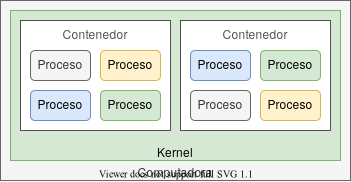
\includegraphics[width=.45\linewidth]{images/diagrams/docker.png}
	\caption{Diagrama del contenedor de procesos Docker.}
	\label{fig:docker_diagrama}
\end{figure}

\subsubsection{Masonite ORM}

Masonite ORM es una solución creada para python que permite la manipulación de sistemas relacionales de bases de datos creando una interfaz de código. Abstrae la complejidad de la manipulación de base de datos para convertirla en un modelo de clases con una interfaz simple para la edición de los datos. Tiene soporte nativo para transacciones, es compatible con MariaDB y está diseñado para ser incluido en proyectos complejos sin necesidad de incluir un framework completo\cite{masonite_2021}.

\subsubsection{FastAPI}

FastAPI es un framework para desarrollo de APIs REST para Python centrado en el desarrollo rápido con ayuda de las anotaciones estándar de Python. Además de ser uno de los frameworks de desarrollo más rápidos en su ejecución, permite el crear directamente documentación compatible con el estándar OpenAPI sin necesidad de librerías externas\cite{fastapi_ramirez_2020}. Todo esto lo convierte en un framework ideal para extender proyectos existentes en Python y con su permisiva licencia permite % TODO terminar esta oración

\subsubsection{MariaDB}

MariaDB es un motor de base de datos relacional creado por el equipo original que desarrolló MySQL, es un motor que tiene como objetivo mantenerse completamente abierto y tiene una licencia de uso permisiva para su uso en ambientes comerciales y no comerciales\cite{mariadb_foundation_2019}. Tiene un rendimiento similar a MySQL en operaciones transaccionales, por lo cual es una excelente alternativa cuando se requiere un modelo de licencias permisivo\cite{mariadb_comparison}.

% TODO \subsubsection{React} Sección de tecnología para front, probablemente React

% SNM (Simple management network)
% OpenSource
% RaspberryPI
% Icinga
